In this section we will give an informal introduction of a partizan two-player game played on black-and-white-colored posets. The game is played by removing poset elements of your color, with the result that all greater elements in the poset are removed as well. The game ends when  one of the players has no elements left to remove. This player then loses.
\\
An example of such a game is provided below in Example \ref{ex:game}.
\\
\begin{ex}{}
\label{ex:game}
An example of a partizan element removal game played on a colored poset and an example of gameplay on this game.
\begin{figure}[H]
\centering
$
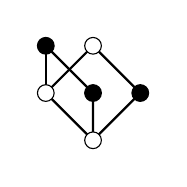
\begin{tikzpicture}[baseline=-0.65ex,scale=.2]
  \draw[thick] (0,-3) -- (-3,0) -- (0,3) -- (3,0) -- (0,-3);
  \draw[thick] (0,-3) -- (0,0) -- (-3,3);
  \draw[thick] (-3,0) -- (-3,3);
  \node (zero) at (0,-3) {\tikz\draw[black,fill=white] (0,0) circle (.7ex);};
  \node (1) at (-3,0) {\tikz\draw[black,fill=white] (0,0) circle (.7ex);};
  \node (2) at (0,0) {\tikz\draw[black,fill=black] (0,0) circle (.7ex);};
  \node (3) at (3,0) {\tikz\draw[black,fill=black] (0,0) circle (.7ex);};
  \node (4) at (-3,3) {\tikz\draw[black,fill=black] (0,0) circle (.7ex);};
  \node (5) at (0,3) {\tikz\draw[black,fill=white] (0,0) circle (.7ex);};
\end{tikzpicture}
=\left\{
\underbrace{
\emptyset
,
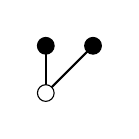
\begin{tikzpicture}[baseline=-0.65ex,scale=.2]
  \draw[thick] (0,-1) -- (3,2);
  \draw[thick] (0,-1) -- (0,2);
  \node (zero) at (0,-1) {\tikz\draw[black,fill=white] (0,0) circle (.7ex);};
  \node (2) at (0,2) {\tikz\draw[black,fill=black] (0,0) circle (.7ex);};
  \node (3) at (3,2) {\tikz\draw[black,fill=black] (0,0) circle (.7ex);};
\end{tikzpicture}
,
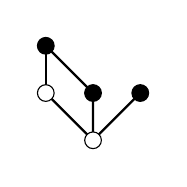
\begin{tikzpicture}[baseline=-0.65ex,scale=.2]
  \draw[thick] (0,-3) -- (-3,0);
  \draw[thick] (0,-3) -- (3,0);
  \draw[thick] (0,-3) -- (0,0) -- (-3,3);
  \draw[thick] (-3,0) -- (-3,3);
  \node (zero) at (0,-3) {\tikz\draw[black,fill=white] (0,0) circle (.7ex);};
  \node (1) at (-3,0) {\tikz\draw[black,fill=white] (0,0) circle (.7ex);};
  \node (2) at (0,0) {\tikz\draw[black,fill=black] (0,0) circle (.7ex);};
  \node (3) at (3,0) {\tikz\draw[black,fill=black] (0,0) circle (.7ex);};
  \node (4) at (-3,3) {\tikz\draw[black,fill=black] (0,0) circle (.7ex);};
\end{tikzpicture}
}_{\text{Left player options}}
\middle|
\underbrace{
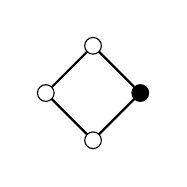
\begin{tikzpicture}[baseline=-0.65ex,scale=.2]
  \draw[thick] (0,-3) -- (-3,0) -- (0,3) -- (3,0) -- (0,-3);
  \node (zero) at (0,-3) {\tikz\draw[black,fill=white] (0,0) circle (.7ex);};
  \node (1) at (-3,0) {\tikz\draw[black,fill=white] (0,0) circle (.7ex);};
  \node (3) at (3,0) {\tikz\draw[black,fill=black] (0,0) circle (.7ex);};
  \node (5) at (0,3) {\tikz\draw[black,fill=white] (0,0) circle (.7ex);};
\end{tikzpicture}
,
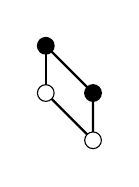
\begin{tikzpicture}[baseline=-0.65ex,scale=.2]
  \draw[thick] (0,-3) -- (-3,0);
  \draw[thick] (0,-3) -- (0,0) -- (-3,3);
  \draw[thick] (-3,0) -- (-3,3);
  \node (zero) at (0,-3) {\tikz\draw[black,fill=white] (0,0) circle (.7ex);};
  \node (1) at (-3,0) {\tikz\draw[black,fill=white] (0,0) circle (.7ex);};
  \node (2) at (0,0) {\tikz\draw[black,fill=black] (0,0) circle (.7ex);};
  \node (4) at (-3,3) {\tikz\draw[black,fill=black] (0,0) circle (.7ex);};
\end{tikzpicture}
,
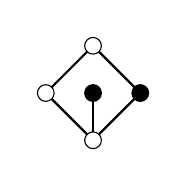
\begin{tikzpicture}[baseline=-0.65ex,scale=.2]
  \draw[thick] (0,-3) -- (-3,0) -- (0,3) -- (3,0) -- (0,-3);
  \draw[thick] (0,-3) -- (0,0);
  \node (zero) at (0,-3) {\tikz\draw[black,fill=white] (0,0) circle (.7ex);};
  \node (1) at (-3,0) {\tikz\draw[black,fill=white] (0,0) circle (.7ex);};
  \node (2) at (0,0) {\tikz\draw[black,fill=black] (0,0) circle (.7ex);};
  \node (3) at (3,0) {\tikz\draw[black,fill=black] (0,0) circle (.7ex);};
  \node (5) at (0,3) {\tikz\draw[black,fill=white] (0,0) circle (.7ex);};
\end{tikzpicture}
}_{\text{Right player options}}
\right\}
$
\caption{Example of a colored poset element removal game.}
\label{fig:posetgameex}
\end{figure}
\begin{figure}[H]
\centering
$
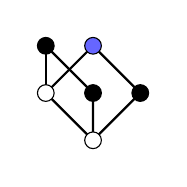
\begin{tikzpicture}[baseline=-0.65ex,scale=.2]
  \draw[thick] (0,-3) -- (-3,0) -- (0,3) -- (3,0) -- (0,-3);
  \draw[thick] (0,-3) -- (0,0) -- (-3,3);
  \draw[thick] (-3,0) -- (-3,3);
  \node (zero) at (0,-3) {\tikz\draw[black,fill=white] (0,0) circle (.7ex);};
  \node (1) at (-3,0) {\tikz\draw[black,fill=white] (0,0) circle (.7ex);};
  \node (2) at (0,0) {\tikz\draw[black,fill=black] (0,0) circle (.7ex);};
  \node (3) at (3,0) {\tikz\draw[black,fill=black] (0,0) circle (.7ex);};
  \node (4) at (-3,3) {\tikz\draw[black,fill=black] (0,0) circle (.7ex);};
  \node (5) at (0,3) {\tikz\draw[black,fill=blue!60] (0,0) circle (.7ex);};
\end{tikzpicture}
\overset{L}{\longrightarrow}
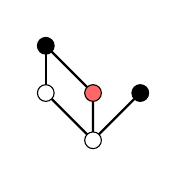
\begin{tikzpicture}[baseline=-0.65ex,scale=.2]
  \draw[thick] (0,-3) -- (-3,0);
  \draw[thick] (0,-3) -- (3,0);
  \draw[thick] (0,-3) -- (0,0) -- (-3,3);
  \draw[thick] (-3,0) -- (-3,3);
  \node (zero) at (0,-3) {\tikz\draw[black,fill=white] (0,0) circle (.7ex);};
  \node (1) at (-3,0) {\tikz\draw[black,fill=white] (0,0) circle (.7ex);};
  \node (2) at (0,0) {\tikz\draw[black,fill=red!60] (0,0) circle (.7ex);};
  \node (3) at (3,0) {\tikz\draw[black,fill=black] (0,0) circle (.7ex);};
  \node (4) at (-3,3) {\tikz\draw[black,fill=black] (0,0) circle (.7ex);};
\end{tikzpicture}
\overset{R}{\longrightarrow}
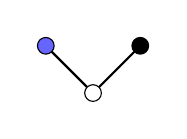
\begin{tikzpicture}[baseline=-0.65ex,scale=.2]
  \draw[thick] (0,-3) -- (-3,0);
  \draw[thick] (0,-3) -- (3,0);
  \node (zero) at (0,-3) {\tikz\draw[black,fill=white] (0,0) circle (.7ex);};
  \node (1) at (-3,0) {\tikz\draw[black,fill=blue!60] (0,0) circle (.7ex);};
  \node (3) at (3,0) {\tikz\draw[black,fill=black] (0,0) circle (.7ex);};
\end{tikzpicture}
\overset{L}{\longrightarrow}
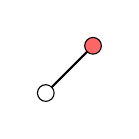
\begin{tikzpicture}[baseline=-0.65ex,scale=.2]
  \draw[thick] (0,-3) -- (3,0);
  \node (zero) at (0,-3) {\tikz\draw[black,fill=white] (0,0) circle (.7ex);};
  \node (3) at (3,0) {\tikz\draw[black,fill=red!60] (0,0) circle (.7ex);};
\end{tikzpicture}
\overset{R}{\longrightarrow}
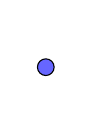
\begin{tikzpicture}[baseline=-0.65ex,scale=.2]
  \node (zero) at (0,-3) {\tikz\draw[black,fill=blue!60] (0,0) circle (.7ex);};
\end{tikzpicture}
\overset{L}{\longrightarrow}
%\emptyset
$
\caption{Example of gameplay on the game in Figure \ref{fig:posetgameex} where Left player wins. Play moves are highlighted with blue (Left) and red (Right).}
\end{figure}
\end{ex}
~\\
In particular, this thesis will focus on games played on \emph{chess-colored} posets, where the posets are in the form of \emph{Young diagrams}. An example of a chess-colored Young diagram and a game played on this Young diagram is provided in Example \ref{ex:younggameplay}.
\begin{ex}{}
\label{ex:younggameplay}
An example of a chess-colored Young diagram and an example of a gameplay on this Young diagram.
\begin{figure}[H]
\centering
\begin{tabular}{ | c | c | c | c | c | c | c |}
\hline
~&\cellcolor[gray]{0}&~&\cellcolor[gray]{0}&~&\cellcolor[gray]{0}&~\\
\hline
\cellcolor[gray]{0}&~&\cellcolor[gray]{0}&~&\cellcolor[gray]{0}\\
\cline{1-5}
~&\cellcolor[gray]{0}\\
\cline{1-2}
\cellcolor[gray]{0}&~\\
\cline{1-2}
~\\
\cline{1-1}
\end{tabular}
\captionof{figure}{Example of a chess-colored Young diagram.}
\label{fig:chessyoungex}
\end{figure}
\begin{figure}[H]
\centering
$
\begin{tabular}{ | c | c | c | c | c | c | c |}
\hline
~&\cellcolor[gray]{0}&~&\cellcolor[gray]{0}&\cellcolor{blue!60}&\cellcolor[gray]{0}&~\\
\hline
\cellcolor[gray]{0}&~&\cellcolor[gray]{0}&~&\cellcolor[gray]{0}\\
\cline{1-5}
~&\cellcolor[gray]{0}\\
\cline{1-2}
\cellcolor[gray]{0}&~\\
\cline{1-2}
~\\
\cline{1-1}
\end{tabular}
\overset{L}{\longrightarrow}
\begin{tabular}{ | c | c | c | c |}
\hline
~&\cellcolor[gray]{0}&~&\cellcolor[gray]{0}\\
\hline
\cellcolor{red!60}&~&\cellcolor[gray]{0}&~\\
\cline{1-4}
~&\cellcolor[gray]{0}\\
\cline{1-2}
\cellcolor[gray]{0}&~\\
\cline{1-2}
~\\
\cline{1-1}
\end{tabular}
\overset{R}{\longrightarrow}
\begin{tabular}{ | c | c | c | c |}
\hline
\cellcolor{blue!60}&\cellcolor[gray]{0}&~&\cellcolor[gray]{0}\\
\hline
\end{tabular}
\overset{L}{\longrightarrow}
\emptyset
$
\captionof{figure}{Example of gameplay on the chess-colored Young diagram of Figure \ref{fig:chessyoungex} where Left player wins. Play moves are highlighted with blue (Left) and red (Right).}
\label{fig:chessyounggameplay}
\end{figure}
\end{ex}
~\\
For these games in general, we will show that they are all surreal numbers, and that, given some properties, they always are valued between 0 and 1. %We will also show that games played on \emph{forest posets} are equivalent to games of \emph{Blue-Red Hackenbush}.
\\
Finally, for games played on chess-colored Young diagrams with $\le3$ rows, we will show that the value is easy to compute by proving that they can be computed with a given formula.
\\\\
First a brief background of poset games will be covered.
\subsection{Background}
A poset game is an element-removal game played on a poset, where a player selects an element and removes this element and all greater elements. A poset game can be both impartial (if it is not colored) and partizan (if it is colored, i.e., each element has a color which specifies who can select and remove it). It is known that the problem of deciding the winner of an impartial uncolored poset game is \textsf{PSPACE}-complete\cite{grier2013}.
\\\\
The simplest possible impartial poset game is the one played on a collection of one-dimensional chain posets, also known as \emph{Nim}. The game of Nim is played by removing a number of elements from one of multiple piles of elements. The player removing the last element wins the game. For a more intuitive understanding of Nim, an example of a gameplay on a game of Nim is provided in Example \ref{ex:nim}.
\begin{ex}{}
\label{ex:nim}
An example gameplay on a game of Nim.
\begin{figure}[H]
\centering
$
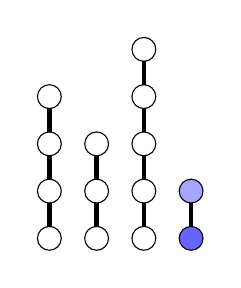
\begin{tikzpicture}[baseline=-0.65ex,scale=.2]
  \draw[ultra thick] (-2,-3) -- (-2,6);
  \draw[ultra thick] (1,-3) -- (1,3);
  \draw[ultra thick] (4,-3) -- (4,9);
  \draw[ultra thick] (7,-3) -- (7,0);
  \node (11) at (-2,-3) {\tikz\draw[black,fill=white] (0,0) circle (1ex);};
  \node (12) at (-2,0) {\tikz\draw[black,fill=white] (0,0) circle (1ex);};
  \node (13) at (-2,3) {\tikz\draw[black,fill=white] (0,0) circle (1ex);};
  \node (14) at (-2,6) {\tikz\draw[black,fill=white] (0,0) circle (1ex);};
  \node (21) at (1,-3) {\tikz\draw[black,fill=white] (0,0) circle (1ex);};
  \node (22) at (1,0) {\tikz\draw[black,fill=white] (0,0) circle (1ex);};
  \node (23) at (1,3) {\tikz\draw[black,fill=white] (0,0) circle (1ex);};
  \node (31) at (4,-3) {\tikz\draw[black,fill=white] (0,0) circle (1ex);};
  \node (32) at (4,0) {\tikz\draw[black,fill=white] (0,0) circle (1ex);};
  \node (33) at (4,3) {\tikz\draw[black,fill=white] (0,0) circle (1ex);};
  \node (34) at (4,6) {\tikz\draw[black,fill=white] (0,0) circle (1ex);};
  \node (35) at (4,9) {\tikz\draw[black,fill=white] (0,0) circle (1ex);};
  \node (41) at (7,-3) {\tikz\draw[black,fill=blue!60] (0,0) circle (1ex);};
  \node (42) at (7,0) {\tikz\draw[black,fill=blue!35] (0,0) circle (1ex);};
\end{tikzpicture}
\overset{L}{\longrightarrow}
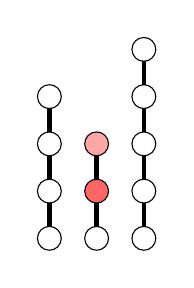
\begin{tikzpicture}[baseline=-0.65ex,scale=.2]
  \draw[ultra thick] (-2,-3) -- (-2,6);
  \draw[ultra thick] (1,-3) -- (1,3);
  \draw[ultra thick] (4,-3) -- (4,9);
  \node (11) at (-2,-3) {\tikz\draw[black,fill=white] (0,0) circle (1ex);};
  \node (12) at (-2,0) {\tikz\draw[black,fill=white] (0,0) circle (1ex);};
  \node (13) at (-2,3) {\tikz\draw[black,fill=white] (0,0) circle (1ex);};
  \node (14) at (-2,6) {\tikz\draw[black,fill=white] (0,0) circle (1ex);};
  \node (21) at (1,-3) {\tikz\draw[black,fill=white] (0,0) circle (1ex);};
  \node (22) at (1,0) {\tikz\draw[black,fill=red!60] (0,0) circle (1ex);};
  \node (23) at (1,3) {\tikz\draw[black,fill=red!35] (0,0) circle (1ex);};
  \node (31) at (4,-3) {\tikz\draw[black,fill=white] (0,0) circle (1ex);};
  \node (32) at (4,0) {\tikz\draw[black,fill=white] (0,0) circle (1ex);};
  \node (33) at (4,3) {\tikz\draw[black,fill=white] (0,0) circle (1ex);};
  \node (34) at (4,6) {\tikz\draw[black,fill=white] (0,0) circle (1ex);};
  \node (35) at (4,9) {\tikz\draw[black,fill=white] (0,0) circle (1ex);};
\end{tikzpicture}
\overset{R}{\longrightarrow}
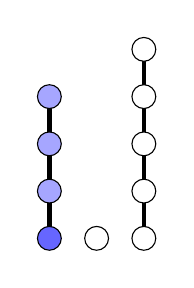
\begin{tikzpicture}[baseline=-0.65ex,scale=.2]
  \draw[ultra thick] (-2,-3) -- (-2,6);
  \draw[ultra thick] (4,-3) -- (4,9);
  \node (11) at (-2,-3) {\tikz\draw[black,fill=blue!60] (0,0) circle (1ex);};
  \node (12) at (-2,0) {\tikz\draw[black,fill=blue!35] (0,0) circle (1ex);};
  \node (13) at (-2,3) {\tikz\draw[black,fill=blue!35] (0,0) circle (1ex);};
  \node (14) at (-2,6) {\tikz\draw[black,fill=blue!35] (0,0) circle (1ex);};
  \node (21) at (1,-3) {\tikz\draw[black,fill=white] (0,0) circle (1ex);};
  \node (31) at (4,-3) {\tikz\draw[black,fill=white] (0,0) circle (1ex);};
  \node (32) at (4,0) {\tikz\draw[black,fill=white] (0,0) circle (1ex);};
  \node (33) at (4,3) {\tikz\draw[black,fill=white] (0,0) circle (1ex);};
  \node (34) at (4,6) {\tikz\draw[black,fill=white] (0,0) circle (1ex);};
  \node (35) at (4,9) {\tikz\draw[black,fill=white] (0,0) circle (1ex);};
\end{tikzpicture}
\overset{L}{\longrightarrow}
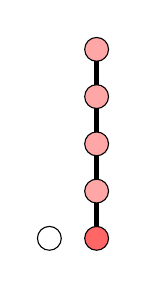
\begin{tikzpicture}[baseline=-0.65ex,scale=.2]
  \draw[ultra thick] (4,-3) -- (4,9);
  \node (21) at (1,-3) {\tikz\draw[black,fill=white] (0,0) circle (1ex);};
  \node (31) at (4,-3) {\tikz\draw[black,fill=red!60] (0,0) circle (1ex);};
  \node (32) at (4,0) {\tikz\draw[black,fill=red!35] (0,0) circle (1ex);};
  \node (33) at (4,3) {\tikz\draw[black,fill=red!35] (0,0) circle (1ex);};
  \node (34) at (4,6) {\tikz\draw[black,fill=red!35] (0,0) circle (1ex);};
  \node (35) at (4,9) {\tikz\draw[black,fill=red!35] (0,0) circle (1ex);};
\end{tikzpicture}
\overset{R}{\longrightarrow}
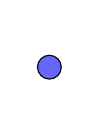
\begin{tikzpicture}[baseline=-0.65ex,scale=.2]
  \node (21) at (0,-3) {\tikz\draw[black,fill=blue!60] (0,0) circle (1ex);};
\end{tikzpicture}
\overset{L}{\longrightarrow}
\begin{tikzpicture}[baseline=-0.0ex]
  \node at (0,-0.55) {$\emptyset$};
\end{tikzpicture}
%\emptyset
$
\caption{Example of gameplay on a game of Nim where Left player wins. Play moves are highlighted with blue (Left) and red (Right).}
\end{figure}
\end{ex}
~\\
Another impartial poset game is the game \emph{Chomp}, more thoroughly introduced in Section \ref{section:chomp}. A game of Chomp can be represented by a poset game with a two-dimensional $n\times m$ lattice poset, $n,m>0$ integers, with the bottom element removed, as illustrated in Figure \ref{fig:chompposet}.

\begin{figure}[H]
\centering
\begin{subfigure}{0.25\textwidth}
\begin{tabular}{ | c | c | c | c | c |}
\hline
~&~&~&~&~\\
\hline
~&~&~&~&~\\
\hline
~&~&~&~&~\\
\hline
~&~&~&~&~\\
\hline
~&~&~&~&~\\
\hline
~&~&~&~&~\\
\hline
\cellcolor{red}&~&~&~&~\\
\hline
\end{tabular}
\hfill$\Longleftrightarrow$
\end{subfigure}
\begin{subfigure}{0.4\textwidth}
\centering
%\begin{turn}{45}
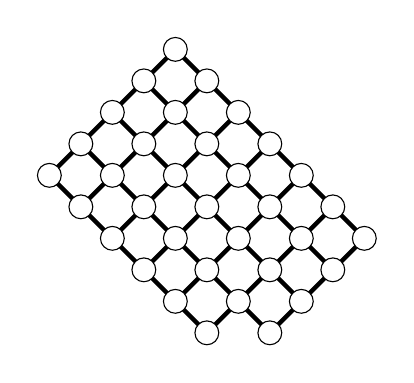
\begin{tikzpicture}[scale=.4]
  \draw[ultra thick] (1,0) -- (4,3);
  \draw[ultra thick] (-1,0) -- (3,4);
  \draw[ultra thick] (-2,1) -- (2,5);
  \draw[ultra thick] (-3,2) -- (1,6);
  \draw[ultra thick] (-4,3) -- (0,7);
  \draw[ultra thick] (-5,4) -- (-1,8);
  \draw[ultra thick] (-6,5) -- (-2,9);
  \draw[ultra thick] (-1,0) -- (-6,5);
  \draw[ultra thick] (1,0) -- (-5,6);
  \draw[ultra thick] (2,1) -- (-4,7);
  \draw[ultra thick] (3,2) -- (-3,8);
  \draw[ultra thick] (4,3) -- (-2,9);
  \node (12) at (1,0) {\tikz\draw[black,fill=white] (0,0) circle (1ex);};
  \node (13) at (2,1) {\tikz\draw[black,fill=white] (0,0) circle (1ex);};
  \node (14) at (3,2) {\tikz\draw[black,fill=white] (0,0) circle (1ex);};
  \node (21) at (4,3) {\tikz\draw[black,fill=white] (0,0) circle (1ex);};
  \node (12) at (-1,0) {\tikz\draw[black,fill=white] (0,0) circle (1ex);};
  \node (12) at (0,1) {\tikz\draw[black,fill=white] (0,0) circle (1ex);};
  \node (13) at (1,2) {\tikz\draw[black,fill=white] (0,0) circle (1ex);};
  \node (14) at (2,3) {\tikz\draw[black,fill=white] (0,0) circle (1ex);};
  \node (21) at (3,4) {\tikz\draw[black,fill=white] (0,0) circle (1ex);};
  \node (12) at (-2,1) {\tikz\draw[black,fill=white] (0,0) circle (1ex);};
  \node (12) at (-1,2) {\tikz\draw[black,fill=white] (0,0) circle (1ex);};
  \node (13) at (0,3) {\tikz\draw[black,fill=white] (0,0) circle (1ex);};
  \node (14) at (1,4) {\tikz\draw[black,fill=white] (0,0) circle (1ex);};
  \node (21) at (2,5) {\tikz\draw[black,fill=white] (0,0) circle (1ex);};
  \node (12) at (-3,2) {\tikz\draw[black,fill=white] (0,0) circle (1ex);};
  \node (12) at (-2,3) {\tikz\draw[black,fill=white] (0,0) circle (1ex);};
  \node (13) at (-1,4) {\tikz\draw[black,fill=white] (0,0) circle (1ex);};
  \node (14) at (0,5) {\tikz\draw[black,fill=white] (0,0) circle (1ex);};
  \node (21) at (1,6) {\tikz\draw[black,fill=white] (0,0) circle (1ex);};
  \node (12) at (-4,3) {\tikz\draw[black,fill=white] (0,0) circle (1ex);};
  \node (12) at (-3,4) {\tikz\draw[black,fill=white] (0,0) circle (1ex);};
  \node (13) at (-2,5) {\tikz\draw[black,fill=white] (0,0) circle (1ex);};
  \node (14) at (-1,6) {\tikz\draw[black,fill=white] (0,0) circle (1ex);};
  \node (21) at (0,7) {\tikz\draw[black,fill=white] (0,0) circle (1ex);};
  \node (12) at (-5,4) {\tikz\draw[black,fill=white] (0,0) circle (1ex);};
  \node (12) at (-4,5) {\tikz\draw[black,fill=white] (0,0) circle (1ex);};
  \node (13) at (-3,6) {\tikz\draw[black,fill=white] (0,0) circle (1ex);};
  \node (14) at (-2,7) {\tikz\draw[black,fill=white] (0,0) circle (1ex);};
  \node (21) at (-1,8) {\tikz\draw[black,fill=white] (0,0) circle (1ex);};
  \node (12) at (-6,5) {\tikz\draw[black,fill=white] (0,0) circle (1ex);};
  \node (12) at (-5,6) {\tikz\draw[black,fill=white] (0,0) circle (1ex);};
  \node (13) at (-4,7) {\tikz\draw[black,fill=white] (0,0) circle (1ex);};
  \node (14) at (-3,8) {\tikz\draw[black,fill=white] (0,0) circle (1ex);};
  \node (21) at (-2,9) {\tikz\draw[black,fill=white] (0,0) circle (1ex);};
\end{tikzpicture}
%\end{turn}
\end{subfigure}
\captionof{figure}{A game of Chomp is equivalent to an impartial poset game.}
\label{fig:chompposet}
\end{figure}
While the game of Nim is solved\cite{bouton1901}, i.e., there is a known optimal strategy, there is not so much known about the game of Chomp in general. This also points out how the difficulty can differ for two classes of impartial poset games. Therefore, it is interesting to investigate the properties of \emph{partizan} poset games, i.e., games on colored posets.
\\
In general, there have been very few studies on partizan poset games. One class of partizan poset games that have been studied are \emph{pomax games}. A pomax game is played on a colored poset, where each player can remove only maximal elements of their own color. Examples of pomax games can be found in Figures \ref{fig:posetpomax} and \ref{fig:youngpomax}.
\begin{figure}[H]
\centering
$
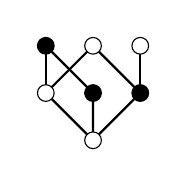
\begin{tikzpicture}[baseline=-0.65ex,scale=.2]
  \draw[thick] (0,-3) -- (-3,0) -- (0,3) -- (3,0) -- (0,-3);
  \draw[thick] (0,-3) -- (0,0) -- (-3,3);
  \draw[thick] (-3,0) -- (-3,3);
  \draw[thick] (3,0) -- (3,3);
  \node (zero) at (0,-3) {\tikz\draw[black,fill=white] (0,0) circle (.7ex);};
  \node (1) at (-3,0) {\tikz\draw[black,fill=white] (0,0) circle (.7ex);};
  \node (2) at (0,0) {\tikz\draw[black,fill=black] (0,0) circle (.7ex);};
  \node (3) at (3,0) {\tikz\draw[black,fill=black] (0,0) circle (.7ex);};
  \node (4) at (-3,3) {\tikz\draw[black,fill=black] (0,0) circle (.7ex);};
  \node (5) at (0,3) {\tikz\draw[black,fill=white] (0,0) circle (.7ex);};
  \node (6) at (3,3) {\tikz\draw[black,fill=white] (0,0) circle (.7ex);};
\end{tikzpicture}
=\left\{
\underbrace{
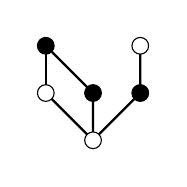
\begin{tikzpicture}[baseline=-0.65ex,scale=.2]
  \draw[thick] (0,-3) -- (-3,0);
  \draw[thick] (0,-3) -- (0,0) -- (-3,3);
  \draw[thick] (-3,0) -- (-3,3);
  \draw[thick] (0,-3) -- (3,0) -- (3,3);
  \node (zero) at (0,-3) {\tikz\draw[black,fill=white] (0,0) circle (.7ex);};
  \node (1) at (-3,0) {\tikz\draw[black,fill=white] (0,0) circle (.7ex);};
  \node (2) at (0,0) {\tikz\draw[black,fill=black] (0,0) circle (.7ex);};
  \node (3) at (3,0) {\tikz\draw[black,fill=black] (0,0) circle (.7ex);};
  \node (4) at (-3,3) {\tikz\draw[black,fill=black] (0,0) circle (.7ex);};
  \node (6) at (3,3) {\tikz\draw[black,fill=white] (0,0) circle (.7ex);};
\end{tikzpicture}
,
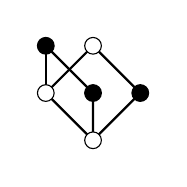
\begin{tikzpicture}[baseline=-0.65ex,scale=.2]
  \draw[thick] (0,-3) -- (-3,0) -- (0,3) -- (3,0) -- (0,-3);
  \draw[thick] (0,-3) -- (0,0) -- (-3,3);
  \draw[thick] (-3,0) -- (-3,3);
  \node (zero) at (0,-3) {\tikz\draw[black,fill=white] (0,0) circle (.7ex);};
  \node (1) at (-3,0) {\tikz\draw[black,fill=white] (0,0) circle (.7ex);};
  \node (2) at (0,0) {\tikz\draw[black,fill=black] (0,0) circle (.7ex);};
  \node (3) at (3,0) {\tikz\draw[black,fill=black] (0,0) circle (.7ex);};
  \node (4) at (-3,3) {\tikz\draw[black,fill=black] (0,0) circle (.7ex);};
  \node (5) at (0,3) {\tikz\draw[black,fill=white] (0,0) circle (.7ex);};
\end{tikzpicture}
}_{\text{Left player options}}
\;\middle|\;
\underbrace{
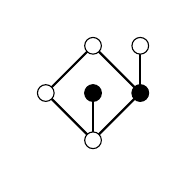
\begin{tikzpicture}[baseline=-0.65ex,scale=.2]
  \draw[thick] (0,-3) -- (-3,0) -- (0,3) -- (3,0) -- (0,-3);
  \draw[thick] (0,-3) -- (0,0);;
  \draw[thick] (3,0) -- (3,3);
  \node (zero) at (0,-3) {\tikz\draw[black,fill=white] (0,0) circle (.7ex);};
  \node (1) at (-3,0) {\tikz\draw[black,fill=white] (0,0) circle (.7ex);};
  \node (2) at (0,0) {\tikz\draw[black,fill=black] (0,0) circle (.7ex);};
  \node (3) at (3,0) {\tikz\draw[black,fill=black] (0,0) circle (.7ex);};
  \node (5) at (0,3) {\tikz\draw[black,fill=white] (0,0) circle (.7ex);};
  \node (6) at (3,3) {\tikz\draw[black,fill=white] (0,0) circle (.7ex);};
\end{tikzpicture}
}_{\text{Right player options}}
\right\}$
\caption{Example of an arbitrary pomax game.}
\label{fig:posetpomax}
\end{figure}
\begin{figure}[H]
\centering
$
\begin{tabular}{ | c | c | c | c | c |}
\hline
~&\cellcolor[gray]{0}&~&\cellcolor[gray]{0}&~\\
\hline
\cellcolor[gray]{0}&~&\cellcolor[gray]{0}\\
\cline{1-3}
~&\cellcolor[gray]{0}\\
\cline{1-2}
\cellcolor[gray]{0}&~\\
\cline{1-2}
\end{tabular}
=\left\{
\underbrace{
\begin{tabular}{ | c | c | c | c |}
\hline
~&\cellcolor[gray]{0}&~&\cellcolor[gray]{0}\\
\hline
\cellcolor[gray]{0}&~&\cellcolor[gray]{0}\\
\cline{1-3}
~&\cellcolor[gray]{0}\\
\cline{1-2}
\cellcolor[gray]{0}&~\\
\cline{1-2}
\end{tabular}
,
\begin{tabular}{ | c | c | c | c | c |}
\hline
~&\cellcolor[gray]{0}&~&\cellcolor[gray]{0}&~\\
\hline
\cellcolor[gray]{0}&~&\cellcolor[gray]{0}\\
\cline{1-3}
~&\cellcolor[gray]{0}\\
\cline{1-2}
\cellcolor[gray]{0}\\
\cline{1-1}
\end{tabular}
}_{\text{Left player options}}
\;\middle|\;
\underbrace{
\begin{tabular}{ | c | c | c | c | c |}
\hline
~&\cellcolor[gray]{0}&~&\cellcolor[gray]{0}&~\\
\hline
\cellcolor[gray]{0}&~\\
\cline{1-2}
~&\cellcolor[gray]{0}\\
\cline{1-2}
\cellcolor[gray]{0}&~\\
\cline{1-2}
\end{tabular}
}_{\text{Right player options}}
\right\}
$
\captionof{figure}{Example of a pomax game on a chess-colored Young diagram.}
\label{fig:youngpomax}
\end{figure}
It has been shown that all pomax games are integer valued\cite{j2013}, that it is easy to determine the value of pomax games played on trees or on chess-colored Young diagrams\cite{j2013} and that the problem of determining the winner of an arbitrary pomax game is \textsf{PSPACE}-complete\cite{js2014}.
\\\\
This thesis will focus on partizan poset games without the constraint of only being able to remove maximal elements, i.e., more similar to the gameplay of the regular poset games, only played on a colored poset. An illustrative example of this type of game is provided in Example \ref{ex:game}.